\documentclass[11pt,a4paper]{article}

% ===================== IDIOMA Y CODIFICACIÓN =====================
\usepackage[utf8]{inputenc}
\usepackage[T1]{fontenc}
% Nombres en español (sin depender del paquete de idioma babel-spanish,
% que no está disponible en algunos entornos de compilación)
\renewcommand{\contentsname}{Índice}
\renewcommand{\figurename}{Figura}
\renewcommand{\tablename}{Tabla}

% ===================== TIPOGRAFÍA: TIMES NEW ROMAN =====================
\usepackage{times}
\usepackage{mathptmx}

% ===================== COLOR: TODO EN NEGRO =====================
\usepackage{xcolor}
\definecolor{black}{RGB}{0,0,0}
\color{black}

% ===================== MÁRGENES =====================
\usepackage[margin=2.5cm]{geometry}

% ===================== TABLAS =====================
\usepackage{array}
\usepackage{longtable}
\usepackage{booktabs}
\renewcommand{\arraystretch}{1.3}

% ===================== DIAGRAMAS =====================
\usepackage{tikz}
\usetikzlibrary{shapes,arrows.meta,positioning,calc,fit,backgrounds}
\usepackage[export]{adjustbox}

% ===================== IMÁGENES (capturas del SGA) =====================
\usepackage{graphicx}

% ===================== HIPERVÍNCULOS SIN COLOR =====================
\usepackage[hidelinks]{hyperref}
\hypersetup{
    colorlinks=false,
    pdfborder={0 0 0},
    pdftitle={Prueba Práctica Unidad IV - ISR-401},
    pdfauthor={Mesias Quijije Jhon Alexander}
}

% ===================== TÍTULOS: NEGRITA, SIN RAYAS =====================
\usepackage{titlesec}
\titleformat{\section}
    {\normalfont\Large\bfseries\color{black}}
    {\thesection.}{0.5em}{}
\titleformat{\subsection}
    {\normalfont\large\bfseries\color{black}}
    {\thesubsection.}{0.5em}{}
\titleformat{\subsubsection}
    {\normalfont\normalsize\bfseries\color{black}}
    {\thesubsubsection.}{0.5em}{}
\titlespacing*{\section}{0pt}{3.5ex plus 1ex minus .2ex}{2ex}
\titlespacing*{\subsection}{0pt}{2.5ex plus 1ex minus .2ex}{1.5ex}

% ===================== ITEMIZE / ENUMERATE =====================
\usepackage{enumitem}
\setlist[itemize]{leftmargin=*}
\setlist[enumerate]{leftmargin=*}

% ===================== ENCABEZADOS DE PÁGINA =====================
\usepackage{fancyhdr}
\pagestyle{fancy}
\fancyhf{}
\renewcommand{\headrulewidth}{0pt}
\renewcommand{\footrulewidth}{0pt}
\fancyfoot[C]{\thepage}
\fancyhead[L]{\small ISR-401 -- Prueba Práctica Unidad IV}
\fancyhead[R]{\small Sistema de Gestión de Pedidos}

\begin{document}

% =========================================================
% CARÁTULA
% =========================================================
\begin{titlepage}
\begin{center}
\vspace*{1.5cm}

{\Large\bfseries UNIVERSIDAD TÉCNICA ESTATAL DE QUEVEDO}\\[0.3cm]
{\large\bfseries FACULTAD DE CIENCIAS DE LA INGENIERÍA}\\[0.2cm]
{\large\bfseries CARRERA DE INGENIERÍA EN SOFTWARE}\\[2cm]

{\LARGE\bfseries PRUEBA PRÁCTICA -- UNIDAD IV}\\[0.4cm]
{\Large\bfseries INGENIERÍA DE REQUISITOS (ISR-401)}\\[0.4cm]
{\large\bfseries Caso: Sistema de Gestión de Pedidos}\\[2cm]

\begin{tabular}{lp{9cm}}
\textbf{Docente:} & Ing. Gleiston Cicerón Guerrero Ulloa, PhD \\[0.3cm]
\textbf{Estudiante:} & Mesias Quijije Jhon Alexander \\[0.3cm]
\textbf{Asignatura:} & Ingeniería de Requisitos -- ISR-401 \\[0.3cm]
\textbf{Semestre:} & Cuarto Semestre \\[0.3cm]
\textbf{Repositorio GitHub:} & \small\url{https://github.com/jhonaelx24/Evaluaci-n-Pr-ctica-de-la-Unidad-IV} \\
\end{tabular}

\vfill

\vspace{1cm}
{\large\bfseries Quevedo -- Los Ríos -- Ecuador}\\
{\large 2026}

\end{center}
\end{titlepage}

\tableofcontents
\newpage

% =========================================================
% P1
% =========================================================
\section{Modelo de datos -- Diagrama de clases UML}

\subsection*{Clases y atributos}
\begin{itemize}
    \item \textbf{Cliente}: cédulaRUC: String [id], nombre: String, correo: String -- \texttt{+registrarPedido()}
    \item \textbf{Pedido}: idPedido: String [id], fecha: Date, total: Decimal -- \texttt{+confirmar()}, \texttt{+despachar()}, \texttt{+entregar()}, \texttt{+anular()}
    \item \textbf{LíneaPedido}: cantidad: int, subtotal: Decimal -- \texttt{+calcularSubtotal()}
    \item \textbf{Producto}: código: String [id], descripción: String, precio: Decimal, stock: int -- \texttt{+verificarStock()}
\end{itemize}

\subsection*{Asociaciones y multiplicidades}
\begin{itemize}
    \item Cliente 1 --- 0..* Pedido
    \item Pedido 1 --- 1..* LíneaPedido (composición)
    \item LíneaPedido 0..* --- 1 Producto
\end{itemize}

\subsection*{Diagrama de clases}
\begin{figure}[h!]
    \centering
    \resizebox{0.95\textwidth}{!}{% ============================================================
% class_diagram.tex
% Diagrama de clases UML — Sistema de Gestión de Pedidos (P1)
% ISR-401 — Prueba Práctica Unidad IV
% ============================================================
% Este archivo puede compilarse de forma independiente o
% incluirse desde main.tex con % ============================================================
% class_diagram.tex
% Diagrama de clases UML — Sistema de Gestión de Pedidos (P1)
% ISR-401 — Prueba Práctica Unidad IV
% ============================================================
% Este archivo puede compilarse de forma independiente o
% incluirse desde main.tex con % ============================================================
% class_diagram.tex
% Diagrama de clases UML — Sistema de Gestión de Pedidos (P1)
% ISR-401 — Prueba Práctica Unidad IV
% ============================================================
% Este archivo puede compilarse de forma independiente o
% incluirse desde main.tex con \input{diagramas/class_diagram}
% ============================================================

\documentclass[tikz,border=10pt]{standalone}
\usepackage{tikz}
\usetikzlibrary{positioning, shapes.multipart, arrows.meta}

\begin{document}
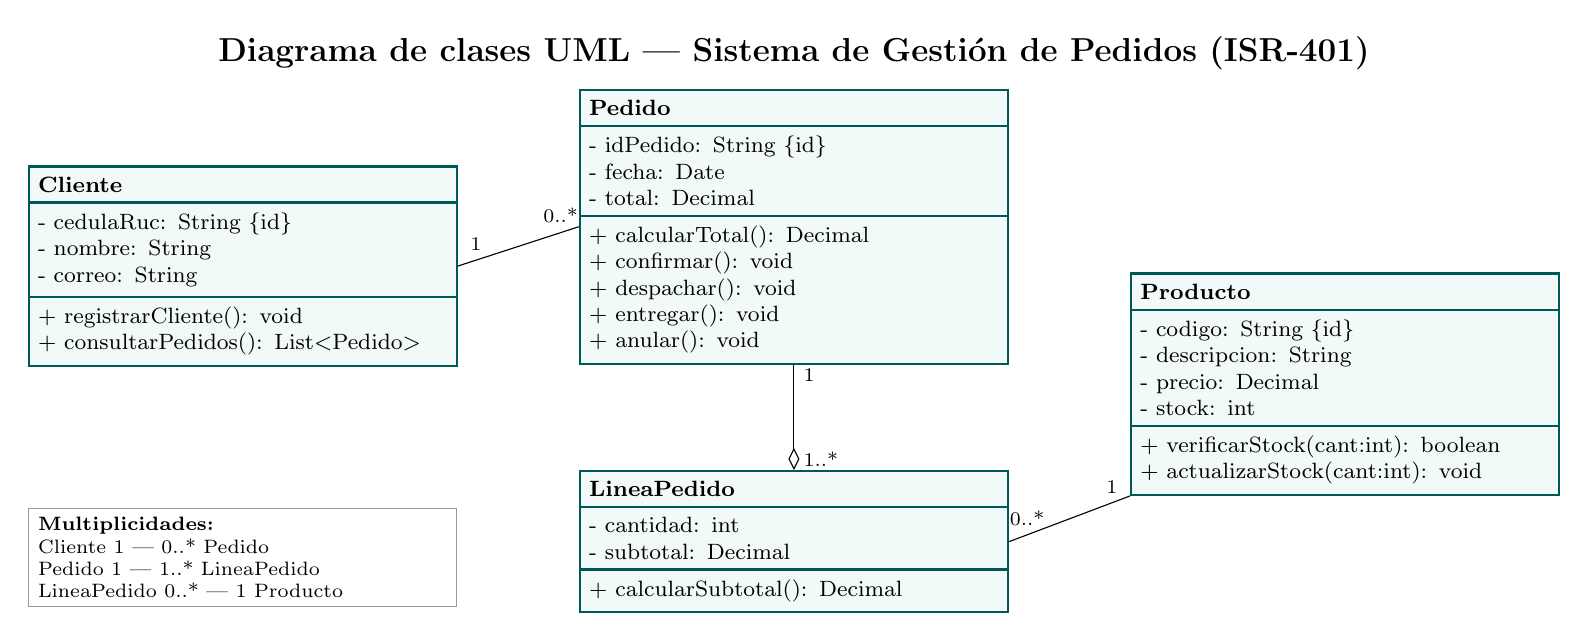
\begin{tikzpicture}[
    class/.style={
        rectangle split, rectangle split parts=3,
        draw=teal!70!black, thick, fill=teal!5,
        rectangle split part align=left,
        text width=5.2cm, font=\footnotesize
    },
    title/.style={font=\bfseries},
    every edge/.style={draw, thick},
    label/.style={font=\scriptsize}
]

% --- Título ---
\node[font=\bfseries\large] at (7,7.7) {Diagrama de clases UML --- Sistema de Gestión de Pedidos (ISR-401)};

% --- Clase Cliente ---
\node[class] (Cliente) at (0,5) {
    \nodepart{one}\textbf{Cliente}
    \nodepart{two}
    - cedulaRuc: String \{id\}\\
    - nombre: String\\
    - correo: String
    \nodepart{three}
    + registrarCliente(): void\\
    + consultarPedidos(): List\textless{}Pedido\textgreater{}
};

% --- Clase Pedido ---
\node[class] (Pedido) at (7,5.5) {
    \nodepart{one}\textbf{Pedido}
    \nodepart{two}
    - idPedido: String \{id\}\\
    - fecha: Date\\
    - total: Decimal
    \nodepart{three}
    + calcularTotal(): Decimal\\
    + confirmar(): void\\
    + despachar(): void\\
    + entregar(): void\\
    + anular(): void
};

% --- Clase LineaPedido ---
\node[class] (LineaPedido) at (7,1.5) {
    \nodepart{one}\textbf{LineaPedido}
    \nodepart{two}
    - cantidad: int\\
    - subtotal: Decimal
    \nodepart{three}
    + calcularSubtotal(): Decimal
};

% --- Clase Producto ---
\node[class] (Producto) at (14,3.5) {
    \nodepart{one}\textbf{Producto}
    \nodepart{two}
    - codigo: String \{id\}\\
    - descripcion: String\\
    - precio: Decimal\\
    - stock: int
    \nodepart{three}
    + verificarStock(cant:int): boolean\\
    + actualizarStock(cant:int): void
};

% --- Asociación Cliente - Pedido ---
\draw[-] (Cliente.east) -- (Pedido.west)
    node[label, pos=0.15, above] {1}
    node[label, pos=0.85, above] {0..*};

% --- Composición Pedido - LineaPedido ---
\draw[-{Diamond[open=false, length=8pt]}] (Pedido.south) -- (LineaPedido.north)
    node[label, pos=0.1, right] {1}
    node[label, pos=0.9, right] {1..*};

% --- Asociación LineaPedido - Producto ---
\draw[-] (LineaPedido.east) -- (Producto.south west)
    node[label, pos=0.15, above] {0..*}
    node[label, pos=0.85, above] {1};

% --- Nota de multiplicidades ---
\node[align=left, font=\scriptsize, draw=black!40, fill=white, text width=5.2cm] at (0,1.3) {
    \textbf{Multiplicidades:}\\
    Cliente 1 --- 0..* Pedido\\
    Pedido 1 --- 1..* LineaPedido\\
    LineaPedido 0..* --- 1 Producto
};

\end{tikzpicture}
\end{document}

% ============================================================

\documentclass[tikz,border=10pt]{standalone}
\usepackage{tikz}
\usetikzlibrary{positioning, shapes.multipart, arrows.meta}

\begin{document}
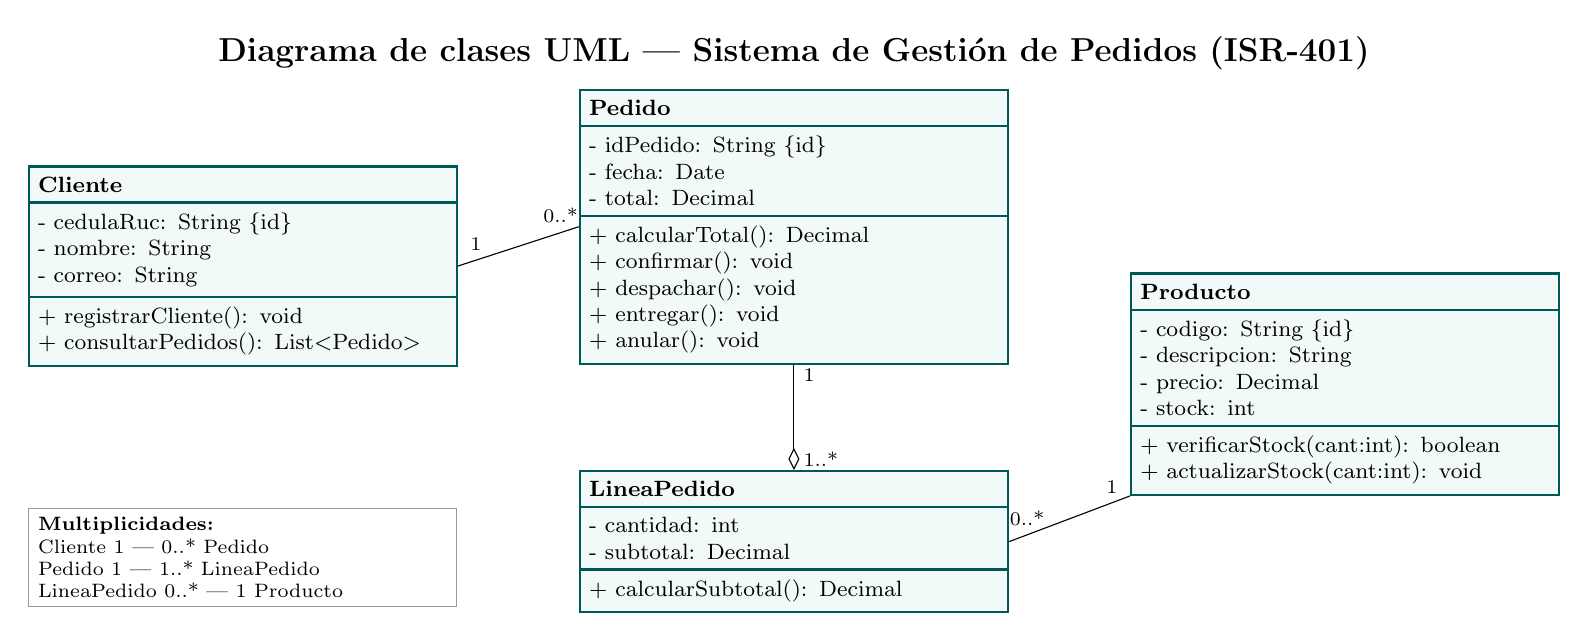
\begin{tikzpicture}[
    class/.style={
        rectangle split, rectangle split parts=3,
        draw=teal!70!black, thick, fill=teal!5,
        rectangle split part align=left,
        text width=5.2cm, font=\footnotesize
    },
    title/.style={font=\bfseries},
    every edge/.style={draw, thick},
    label/.style={font=\scriptsize}
]

% --- Título ---
\node[font=\bfseries\large] at (7,7.7) {Diagrama de clases UML --- Sistema de Gestión de Pedidos (ISR-401)};

% --- Clase Cliente ---
\node[class] (Cliente) at (0,5) {
    \nodepart{one}\textbf{Cliente}
    \nodepart{two}
    - cedulaRuc: String \{id\}\\
    - nombre: String\\
    - correo: String
    \nodepart{three}
    + registrarCliente(): void\\
    + consultarPedidos(): List\textless{}Pedido\textgreater{}
};

% --- Clase Pedido ---
\node[class] (Pedido) at (7,5.5) {
    \nodepart{one}\textbf{Pedido}
    \nodepart{two}
    - idPedido: String \{id\}\\
    - fecha: Date\\
    - total: Decimal
    \nodepart{three}
    + calcularTotal(): Decimal\\
    + confirmar(): void\\
    + despachar(): void\\
    + entregar(): void\\
    + anular(): void
};

% --- Clase LineaPedido ---
\node[class] (LineaPedido) at (7,1.5) {
    \nodepart{one}\textbf{LineaPedido}
    \nodepart{two}
    - cantidad: int\\
    - subtotal: Decimal
    \nodepart{three}
    + calcularSubtotal(): Decimal
};

% --- Clase Producto ---
\node[class] (Producto) at (14,3.5) {
    \nodepart{one}\textbf{Producto}
    \nodepart{two}
    - codigo: String \{id\}\\
    - descripcion: String\\
    - precio: Decimal\\
    - stock: int
    \nodepart{three}
    + verificarStock(cant:int): boolean\\
    + actualizarStock(cant:int): void
};

% --- Asociación Cliente - Pedido ---
\draw[-] (Cliente.east) -- (Pedido.west)
    node[label, pos=0.15, above] {1}
    node[label, pos=0.85, above] {0..*};

% --- Composición Pedido - LineaPedido ---
\draw[-{Diamond[open=false, length=8pt]}] (Pedido.south) -- (LineaPedido.north)
    node[label, pos=0.1, right] {1}
    node[label, pos=0.9, right] {1..*};

% --- Asociación LineaPedido - Producto ---
\draw[-] (LineaPedido.east) -- (Producto.south west)
    node[label, pos=0.15, above] {0..*}
    node[label, pos=0.85, above] {1};

% --- Nota de multiplicidades ---
\node[align=left, font=\scriptsize, draw=black!40, fill=white, text width=5.2cm] at (0,1.3) {
    \textbf{Multiplicidades:}\\
    Cliente 1 --- 0..* Pedido\\
    Pedido 1 --- 1..* LineaPedido\\
    LineaPedido 0..* --- 1 Producto
};

\end{tikzpicture}
\end{document}

% ============================================================

\documentclass[tikz,border=10pt]{standalone}
\usepackage{tikz}
\usetikzlibrary{positioning, shapes.multipart, arrows.meta}

\begin{document}
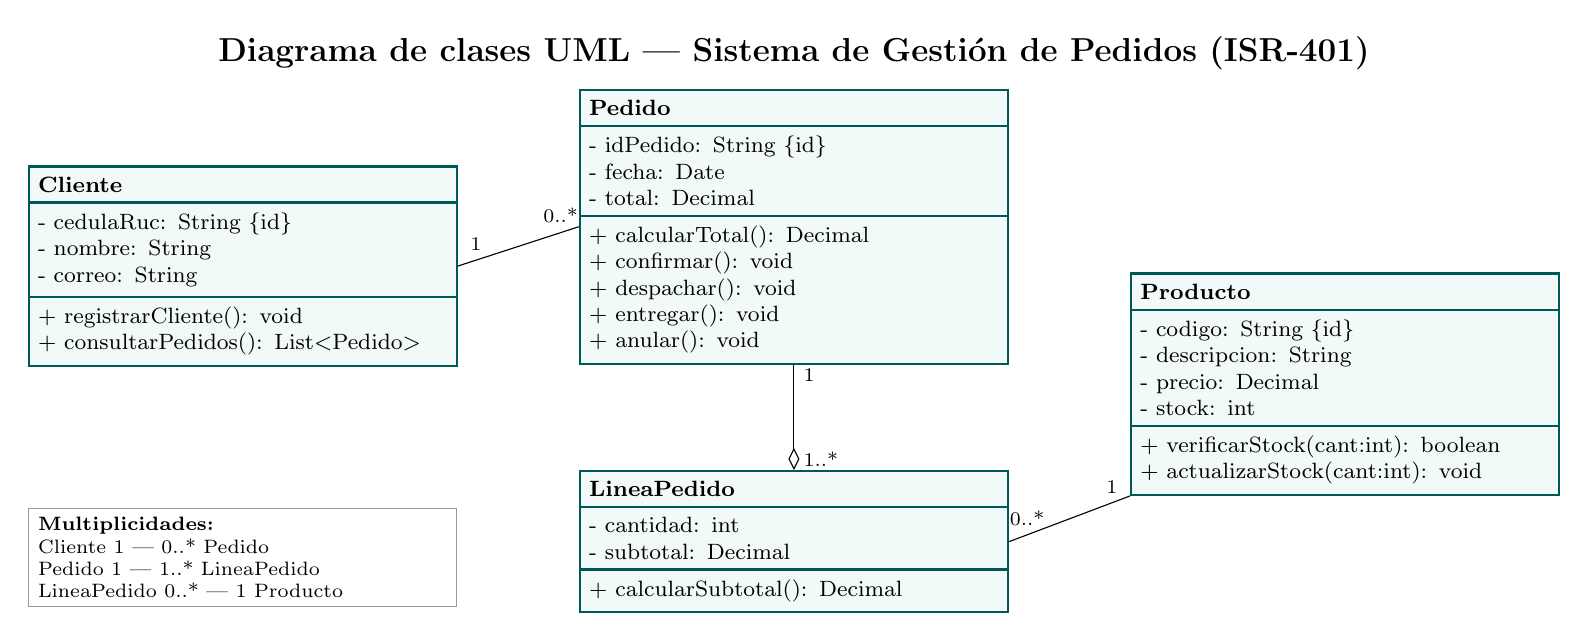
\begin{tikzpicture}[
    class/.style={
        rectangle split, rectangle split parts=3,
        draw=teal!70!black, thick, fill=teal!5,
        rectangle split part align=left,
        text width=5.2cm, font=\footnotesize
    },
    title/.style={font=\bfseries},
    every edge/.style={draw, thick},
    label/.style={font=\scriptsize}
]

% --- Título ---
\node[font=\bfseries\large] at (7,7.7) {Diagrama de clases UML --- Sistema de Gestión de Pedidos (ISR-401)};

% --- Clase Cliente ---
\node[class] (Cliente) at (0,5) {
    \nodepart{one}\textbf{Cliente}
    \nodepart{two}
    - cedulaRuc: String \{id\}\\
    - nombre: String\\
    - correo: String
    \nodepart{three}
    + registrarCliente(): void\\
    + consultarPedidos(): List\textless{}Pedido\textgreater{}
};

% --- Clase Pedido ---
\node[class] (Pedido) at (7,5.5) {
    \nodepart{one}\textbf{Pedido}
    \nodepart{two}
    - idPedido: String \{id\}\\
    - fecha: Date\\
    - total: Decimal
    \nodepart{three}
    + calcularTotal(): Decimal\\
    + confirmar(): void\\
    + despachar(): void\\
    + entregar(): void\\
    + anular(): void
};

% --- Clase LineaPedido ---
\node[class] (LineaPedido) at (7,1.5) {
    \nodepart{one}\textbf{LineaPedido}
    \nodepart{two}
    - cantidad: int\\
    - subtotal: Decimal
    \nodepart{three}
    + calcularSubtotal(): Decimal
};

% --- Clase Producto ---
\node[class] (Producto) at (14,3.5) {
    \nodepart{one}\textbf{Producto}
    \nodepart{two}
    - codigo: String \{id\}\\
    - descripcion: String\\
    - precio: Decimal\\
    - stock: int
    \nodepart{three}
    + verificarStock(cant:int): boolean\\
    + actualizarStock(cant:int): void
};

% --- Asociación Cliente - Pedido ---
\draw[-] (Cliente.east) -- (Pedido.west)
    node[label, pos=0.15, above] {1}
    node[label, pos=0.85, above] {0..*};

% --- Composición Pedido - LineaPedido ---
\draw[-{Diamond[open=false, length=8pt]}] (Pedido.south) -- (LineaPedido.north)
    node[label, pos=0.1, right] {1}
    node[label, pos=0.9, right] {1..*};

% --- Asociación LineaPedido - Producto ---
\draw[-] (LineaPedido.east) -- (Producto.south west)
    node[label, pos=0.15, above] {0..*}
    node[label, pos=0.85, above] {1};

% --- Nota de multiplicidades ---
\node[align=left, font=\scriptsize, draw=black!40, fill=white, text width=5.2cm] at (0,1.3) {
    \textbf{Multiplicidades:}\\
    Cliente 1 --- 0..* Pedido\\
    Pedido 1 --- 1..* LineaPedido\\
    LineaPedido 0..* --- 1 Producto
};

\end{tikzpicture}
\end{document}
}
    \caption{Diagrama de clases UML -- Sistema de Gestión de Pedidos}
    \label{fig:class}
\end{figure}

\newpage

% =========================================================
% P2
% =========================================================
\section{Modelo funcional -- Diagrama de actividades ``Registrar pedido''}

Flujo: Inicio $\rightarrow$ Recibir pedido $\rightarrow$ Verificar stock (nodo de decisión) $\rightarrow$
[Sí] Confirmar pedido $\rightarrow$ Fin $\mid$ [No] Notificar faltante $\rightarrow$ Fin.
Ambos caminos convergen antes del nodo final.

\subsection*{Carriles de responsabilidad sugeridos}
Cliente / Sistema.

\subsection*{Diagrama de actividades}
\begin{figure}[h!]
    \centering
    \resizebox{0.6\textwidth}{!}{% ============================================================
% activity_diagram.tex
% Diagrama de actividades UML — "Registrar pedido" (P2)
% ISR-401 — Prueba Práctica Unidad IV
% ============================================================
% Este archivo puede compilarse de forma independiente o
% incluirse desde main.tex con % ============================================================
% activity_diagram.tex
% Diagrama de actividades UML — "Registrar pedido" (P2)
% ISR-401 — Prueba Práctica Unidad IV
% ============================================================
% Este archivo puede compilarse de forma independiente o
% incluirse desde main.tex con % ============================================================
% activity_diagram.tex
% Diagrama de actividades UML — "Registrar pedido" (P2)
% ISR-401 — Prueba Práctica Unidad IV
% ============================================================
% Este archivo puede compilarse de forma independiente o
% incluirse desde main.tex con \input{diagramas/activity_diagram}
% ============================================================

\documentclass[tikz,border=10pt]{standalone}
\usepackage{tikz}
\usetikzlibrary{shapes.geometric, positioning, arrows.meta}

\begin{document}
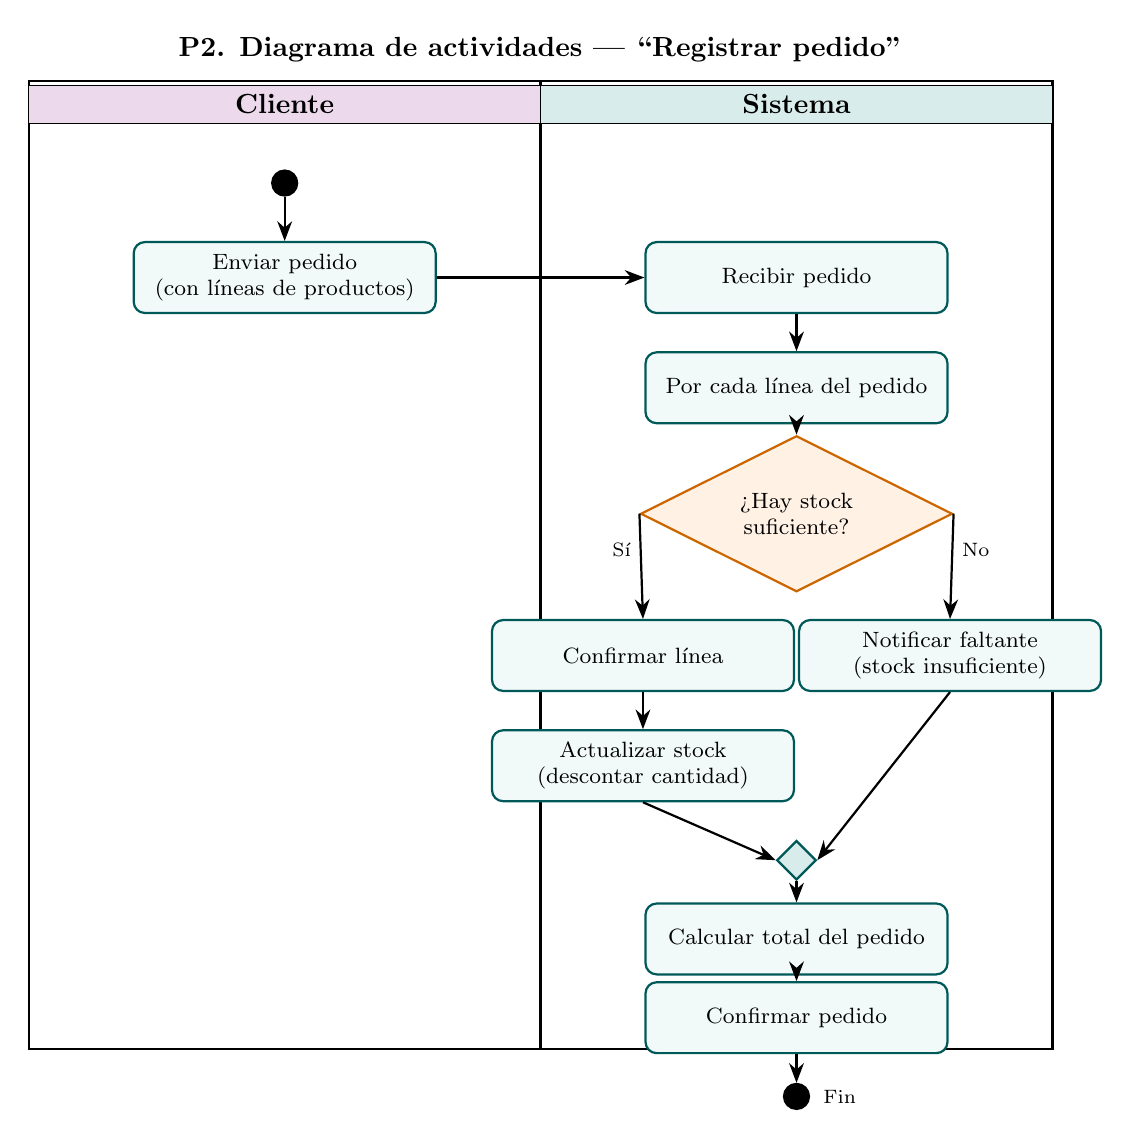
\begin{tikzpicture}[
    action/.style={rectangle, rounded corners, draw=teal!70!black, thick,
        fill=teal!5, text width=3.6cm, align=center, minimum height=0.9cm, font=\footnotesize},
    decision/.style={diamond, draw=orange!80!black, thick, fill=orange!10,
        aspect=2, text width=2.2cm, align=center, font=\footnotesize},
    merge/.style={diamond, draw=teal!70!black, thick, fill=teal!15,
        minimum width=0.5cm, minimum height=0.5cm},
    initial/.style={circle, draw=black, fill=black, minimum size=0.3cm},
    final/.style={circle, draw=black, fill=white, minimum size=0.4cm},
    finaldot/.style={circle, draw=black, fill=black, minimum size=0.2cm},
    swimlane/.style={draw=black, thick, minimum width=6.5cm},
    every edge/.style={draw, -{Stealth[length=2.5mm]}, thick},
    lbl/.style={font=\scriptsize}
]

% --- Título ---
\node[font=\bfseries] at (6.5,12.7) {P2. Diagrama de actividades --- ``Registrar pedido''};

% --- Carriles (swimlanes) ---
\draw[thick] (0,0) rectangle (6.5,12.3);
\draw[thick] (6.5,0) rectangle (13,12.3);
\draw[very thick] (6.5,0) -- (6.5,12.3);

\node[font=\bfseries, fill=violet!15, minimum width=6.5cm, draw] at (3.25,12) {Cliente};
\node[font=\bfseries, fill=teal!15, minimum width=6.5cm, draw] at (9.75,12) {Sistema};

% --- Carril Cliente ---
\node[initial] (ini) at (3.25,11) {};
\node[action] (enviar) at (3.25,9.8) {Enviar pedido\\(con líneas de productos)};

% --- Carril Sistema ---
\node[action] (recibir) at (9.75,9.8) {Recibir pedido};
\node[action] (porcada) at (9.75,8.4) {Por cada línea del pedido};
\node[decision] (hay) at (9.75,6.8) {¿Hay stock suficiente?};

\node[action] (confirmarLinea) at (7.8,5.0) {Confirmar línea};
\node[action] (notificar) at (11.7,5.0) {Notificar faltante\\(stock insuficiente)};

\node[action] (actualizar) at (7.8,3.6) {Actualizar stock\\(descontar cantidad)};

\node[merge] (union) at (9.75,2.4) {};

\node[action] (total) at (9.75,1.4) {Calcular total del pedido};
\node[action] (confirmarPedido) at (9.75,0.4) {Confirmar pedido};

\node[finaldot] (fin) at (9.75,-0.6) {};
\node[lbl] at (10.3,-0.6) {Fin};

% --- Flujo Cliente -> Sistema ---
\draw[-{Stealth[length=2.5mm]}, thick] (ini) -- (enviar);
\draw[-{Stealth[length=2.5mm]}, thick] (enviar.east) -- (recibir.west);

% --- Flujo Sistema ---
\draw[-{Stealth[length=2.5mm]}, thick] (recibir) -- (porcada);
\draw[-{Stealth[length=2.5mm]}, thick] (porcada) -- (hay);

\draw[-{Stealth[length=2.5mm]}, thick] (hay.west) -- (confirmarLinea.north) node[lbl, midway, above left] {Sí};
\draw[-{Stealth[length=2.5mm]}, thick] (hay.east) -- (notificar.north) node[lbl, midway, above right] {No};

\draw[-{Stealth[length=2.5mm]}, thick] (confirmarLinea) -- (actualizar);
\draw[-{Stealth[length=2.5mm]}, thick] (actualizar.south) -- (union.west);
\draw[-{Stealth[length=2.5mm]}, thick] (notificar.south) -- (union.east);

\draw[-{Stealth[length=2.5mm]}, thick] (union) -- (total);
\draw[-{Stealth[length=2.5mm]}, thick] (total) -- (confirmarPedido);
\draw[-{Stealth[length=2.5mm]}, thick] (confirmarPedido) -- (fin);

\end{tikzpicture}
\end{document}

% ============================================================

\documentclass[tikz,border=10pt]{standalone}
\usepackage{tikz}
\usetikzlibrary{shapes.geometric, positioning, arrows.meta}

\begin{document}
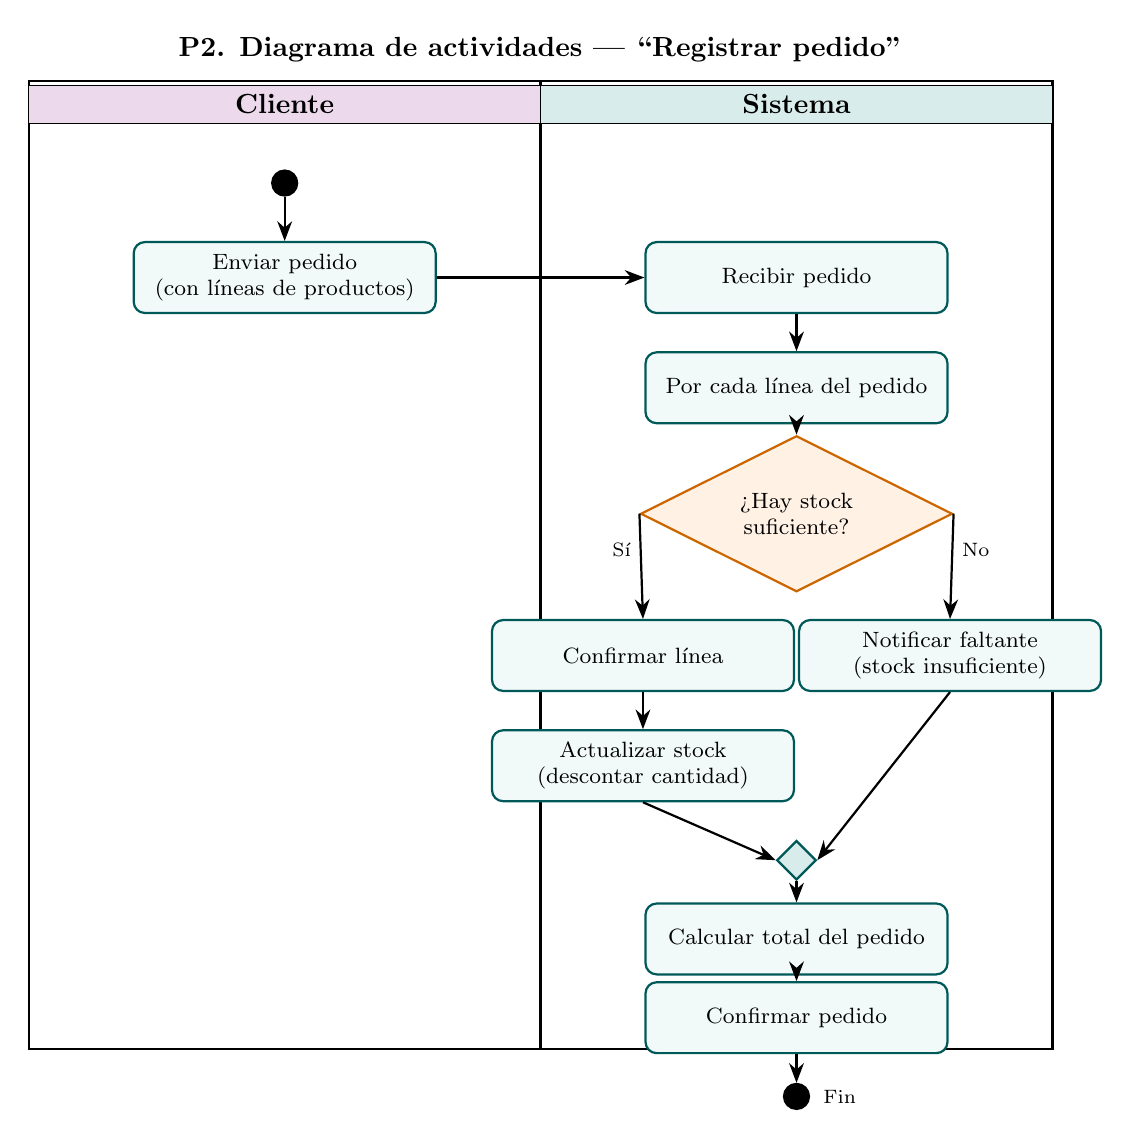
\begin{tikzpicture}[
    action/.style={rectangle, rounded corners, draw=teal!70!black, thick,
        fill=teal!5, text width=3.6cm, align=center, minimum height=0.9cm, font=\footnotesize},
    decision/.style={diamond, draw=orange!80!black, thick, fill=orange!10,
        aspect=2, text width=2.2cm, align=center, font=\footnotesize},
    merge/.style={diamond, draw=teal!70!black, thick, fill=teal!15,
        minimum width=0.5cm, minimum height=0.5cm},
    initial/.style={circle, draw=black, fill=black, minimum size=0.3cm},
    final/.style={circle, draw=black, fill=white, minimum size=0.4cm},
    finaldot/.style={circle, draw=black, fill=black, minimum size=0.2cm},
    swimlane/.style={draw=black, thick, minimum width=6.5cm},
    every edge/.style={draw, -{Stealth[length=2.5mm]}, thick},
    lbl/.style={font=\scriptsize}
]

% --- Título ---
\node[font=\bfseries] at (6.5,12.7) {P2. Diagrama de actividades --- ``Registrar pedido''};

% --- Carriles (swimlanes) ---
\draw[thick] (0,0) rectangle (6.5,12.3);
\draw[thick] (6.5,0) rectangle (13,12.3);
\draw[very thick] (6.5,0) -- (6.5,12.3);

\node[font=\bfseries, fill=violet!15, minimum width=6.5cm, draw] at (3.25,12) {Cliente};
\node[font=\bfseries, fill=teal!15, minimum width=6.5cm, draw] at (9.75,12) {Sistema};

% --- Carril Cliente ---
\node[initial] (ini) at (3.25,11) {};
\node[action] (enviar) at (3.25,9.8) {Enviar pedido\\(con líneas de productos)};

% --- Carril Sistema ---
\node[action] (recibir) at (9.75,9.8) {Recibir pedido};
\node[action] (porcada) at (9.75,8.4) {Por cada línea del pedido};
\node[decision] (hay) at (9.75,6.8) {¿Hay stock suficiente?};

\node[action] (confirmarLinea) at (7.8,5.0) {Confirmar línea};
\node[action] (notificar) at (11.7,5.0) {Notificar faltante\\(stock insuficiente)};

\node[action] (actualizar) at (7.8,3.6) {Actualizar stock\\(descontar cantidad)};

\node[merge] (union) at (9.75,2.4) {};

\node[action] (total) at (9.75,1.4) {Calcular total del pedido};
\node[action] (confirmarPedido) at (9.75,0.4) {Confirmar pedido};

\node[finaldot] (fin) at (9.75,-0.6) {};
\node[lbl] at (10.3,-0.6) {Fin};

% --- Flujo Cliente -> Sistema ---
\draw[-{Stealth[length=2.5mm]}, thick] (ini) -- (enviar);
\draw[-{Stealth[length=2.5mm]}, thick] (enviar.east) -- (recibir.west);

% --- Flujo Sistema ---
\draw[-{Stealth[length=2.5mm]}, thick] (recibir) -- (porcada);
\draw[-{Stealth[length=2.5mm]}, thick] (porcada) -- (hay);

\draw[-{Stealth[length=2.5mm]}, thick] (hay.west) -- (confirmarLinea.north) node[lbl, midway, above left] {Sí};
\draw[-{Stealth[length=2.5mm]}, thick] (hay.east) -- (notificar.north) node[lbl, midway, above right] {No};

\draw[-{Stealth[length=2.5mm]}, thick] (confirmarLinea) -- (actualizar);
\draw[-{Stealth[length=2.5mm]}, thick] (actualizar.south) -- (union.west);
\draw[-{Stealth[length=2.5mm]}, thick] (notificar.south) -- (union.east);

\draw[-{Stealth[length=2.5mm]}, thick] (union) -- (total);
\draw[-{Stealth[length=2.5mm]}, thick] (total) -- (confirmarPedido);
\draw[-{Stealth[length=2.5mm]}, thick] (confirmarPedido) -- (fin);

\end{tikzpicture}
\end{document}

% ============================================================

\documentclass[tikz,border=10pt]{standalone}
\usepackage{tikz}
\usetikzlibrary{shapes.geometric, positioning, arrows.meta}

\begin{document}
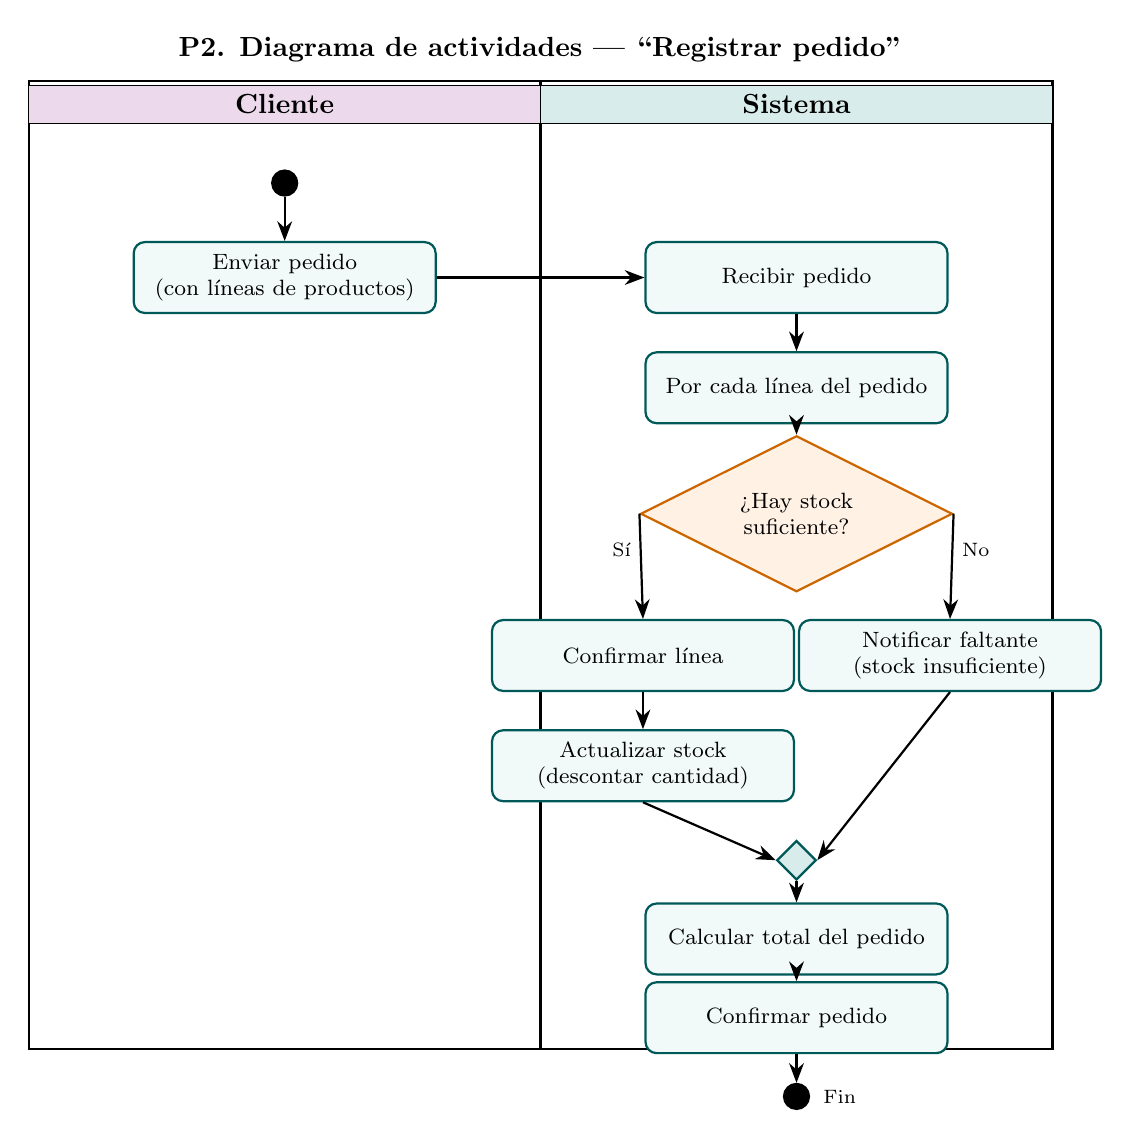
\begin{tikzpicture}[
    action/.style={rectangle, rounded corners, draw=teal!70!black, thick,
        fill=teal!5, text width=3.6cm, align=center, minimum height=0.9cm, font=\footnotesize},
    decision/.style={diamond, draw=orange!80!black, thick, fill=orange!10,
        aspect=2, text width=2.2cm, align=center, font=\footnotesize},
    merge/.style={diamond, draw=teal!70!black, thick, fill=teal!15,
        minimum width=0.5cm, minimum height=0.5cm},
    initial/.style={circle, draw=black, fill=black, minimum size=0.3cm},
    final/.style={circle, draw=black, fill=white, minimum size=0.4cm},
    finaldot/.style={circle, draw=black, fill=black, minimum size=0.2cm},
    swimlane/.style={draw=black, thick, minimum width=6.5cm},
    every edge/.style={draw, -{Stealth[length=2.5mm]}, thick},
    lbl/.style={font=\scriptsize}
]

% --- Título ---
\node[font=\bfseries] at (6.5,12.7) {P2. Diagrama de actividades --- ``Registrar pedido''};

% --- Carriles (swimlanes) ---
\draw[thick] (0,0) rectangle (6.5,12.3);
\draw[thick] (6.5,0) rectangle (13,12.3);
\draw[very thick] (6.5,0) -- (6.5,12.3);

\node[font=\bfseries, fill=violet!15, minimum width=6.5cm, draw] at (3.25,12) {Cliente};
\node[font=\bfseries, fill=teal!15, minimum width=6.5cm, draw] at (9.75,12) {Sistema};

% --- Carril Cliente ---
\node[initial] (ini) at (3.25,11) {};
\node[action] (enviar) at (3.25,9.8) {Enviar pedido\\(con líneas de productos)};

% --- Carril Sistema ---
\node[action] (recibir) at (9.75,9.8) {Recibir pedido};
\node[action] (porcada) at (9.75,8.4) {Por cada línea del pedido};
\node[decision] (hay) at (9.75,6.8) {¿Hay stock suficiente?};

\node[action] (confirmarLinea) at (7.8,5.0) {Confirmar línea};
\node[action] (notificar) at (11.7,5.0) {Notificar faltante\\(stock insuficiente)};

\node[action] (actualizar) at (7.8,3.6) {Actualizar stock\\(descontar cantidad)};

\node[merge] (union) at (9.75,2.4) {};

\node[action] (total) at (9.75,1.4) {Calcular total del pedido};
\node[action] (confirmarPedido) at (9.75,0.4) {Confirmar pedido};

\node[finaldot] (fin) at (9.75,-0.6) {};
\node[lbl] at (10.3,-0.6) {Fin};

% --- Flujo Cliente -> Sistema ---
\draw[-{Stealth[length=2.5mm]}, thick] (ini) -- (enviar);
\draw[-{Stealth[length=2.5mm]}, thick] (enviar.east) -- (recibir.west);

% --- Flujo Sistema ---
\draw[-{Stealth[length=2.5mm]}, thick] (recibir) -- (porcada);
\draw[-{Stealth[length=2.5mm]}, thick] (porcada) -- (hay);

\draw[-{Stealth[length=2.5mm]}, thick] (hay.west) -- (confirmarLinea.north) node[lbl, midway, above left] {Sí};
\draw[-{Stealth[length=2.5mm]}, thick] (hay.east) -- (notificar.north) node[lbl, midway, above right] {No};

\draw[-{Stealth[length=2.5mm]}, thick] (confirmarLinea) -- (actualizar);
\draw[-{Stealth[length=2.5mm]}, thick] (actualizar.south) -- (union.west);
\draw[-{Stealth[length=2.5mm]}, thick] (notificar.south) -- (union.east);

\draw[-{Stealth[length=2.5mm]}, thick] (union) -- (total);
\draw[-{Stealth[length=2.5mm]}, thick] (total) -- (confirmarPedido);
\draw[-{Stealth[length=2.5mm]}, thick] (confirmarPedido) -- (fin);

\end{tikzpicture}
\end{document}
}
    \caption{Diagrama de actividades -- Registrar pedido}
    \label{fig:activity}
\end{figure}

\newpage

% =========================================================
% P3
% =========================================================
\section{Modelo de comportamiento -- Máquina de estados de Pedido}

Registrado --[confirmar / stock disponible]$\rightarrow$ Confirmado --[despachar]$\rightarrow$ Enviado --[entregar]$\rightarrow$ Entregado (estado final).
Desde Confirmado o Enviado: --[anular / no entregado]$\rightarrow$ Cancelado (estado final).

\subsection*{Superestado sugerido}
``Activo'' agrupa \{Confirmado, Enviado\} con una transición de salida ``anular'' común,
factorizando la transición hacia Cancelado.

\subsection*{Diagrama de máquina de estados}
\begin{figure}[h!]
    \centering
    \resizebox{\textwidth}{!}{% ============================================================
% state_diagram.tex
% Máquina de estados UML — Ciclo de vida del Pedido (P3)
% ISR-401 — Prueba Práctica Unidad IV
% ============================================================
% Este archivo puede compilarse de forma independiente o
% incluirse desde main.tex con % ============================================================
% state_diagram.tex
% Máquina de estados UML — Ciclo de vida del Pedido (P3)
% ISR-401 — Prueba Práctica Unidad IV
% ============================================================
% Este archivo puede compilarse de forma independiente o
% incluirse desde main.tex con % ============================================================
% state_diagram.tex
% Máquina de estados UML — Ciclo de vida del Pedido (P3)
% ISR-401 — Prueba Práctica Unidad IV
% ============================================================
% Este archivo puede compilarse de forma independiente o
% incluirse desde main.tex con \input{diagramas/state_diagram}
% ============================================================

\documentclass[tikz,border=10pt]{standalone}
\usepackage{tikz}
\usetikzlibrary{shapes.geometric, positioning, arrows.meta, fit, backgrounds}

\begin{document}
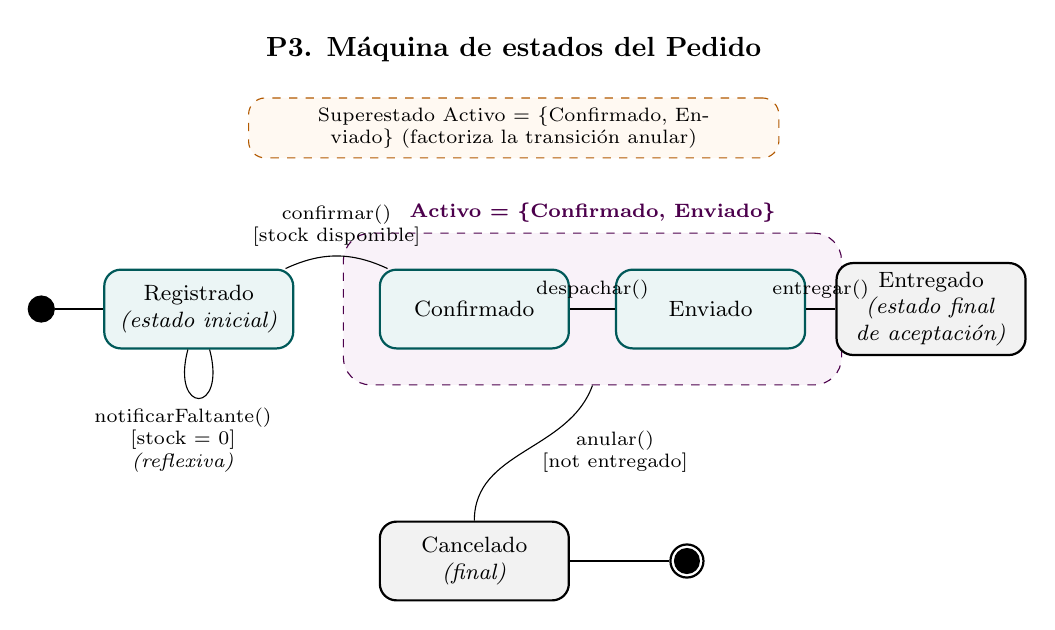
\begin{tikzpicture}[
    state/.style={rectangle, rounded corners=6pt, draw=teal!70!black, thick,
        fill=teal!8, minimum width=2.4cm, minimum height=1cm, align=center, font=\footnotesize},
    finalstate/.style={rectangle, rounded corners=6pt, draw=black, thick,
        fill=gray!10, minimum width=2.4cm, minimum height=1cm, align=center, font=\footnotesize},
    initial/.style={circle, draw=black, fill=black, minimum size=0.3cm},
    finaldot/.style={circle, draw=black, thick, fill=white, minimum size=0.42cm},
    finaldotinner/.style={circle, fill=black, minimum size=0.18cm},
    every edge/.style={draw, -{Stealth[length=2.5mm]}, thick},
    lbl/.style={font=\scriptsize, align=center}
]

% --- Título ---
\node[font=\bfseries] at (6,7.3) {P3. Máquina de estados del Pedido};

% --- Estados principales ---
\node[initial] (ini) at (0,4) {};
\node[state] (registrado) at (2,4) {Registrado\\\textit{(estado inicial)}};
\node[state] (confirmado) at (5.5,4) {Confirmado};
\node[state] (enviado) at (8.5,4) {Enviado};
\node[finalstate] (entregado) at (11.3,4) {Entregado\\\textit{(estado final}\\\textit{de aceptación)}};

\node[finalstate] (cancelado) at (5.5,0.8) {Cancelado\\\textit{(final)}};
\node[finaldot] (finC) at (8.2,0.8) {};
\node[finaldotinner] at (finC) {};

% --- Superestado Activo ---
\begin{scope}[on background layer]
\node[draw=violet!60!black, dashed, rounded corners=10pt, fill=violet!5,
    fit=(confirmado)(enviado), inner sep=0.45cm, label={[font=\scriptsize\bfseries, violet!60!black]above:Activo = \{Confirmado, Enviado\}}] (activo) {};
\end{scope}

\node[draw=orange!70!black, dashed, rounded corners=6pt, fill=orange!5,
    text width=6.5cm, align=center, font=\scriptsize] at (6,6.3)
    {Superestado Activo = \{Confirmado, Enviado\} (factoriza la transición anular)};

% --- Transiciones ---
\draw (ini) -- (registrado);

\draw (registrado) to[bend left=25] node[lbl, above] {confirmar()\\{[stock disponible]}} (confirmado);

\draw (registrado) to[loop below, looseness=8] node[lbl, below, xshift=-0.2cm]
    {notificarFaltante()\\{[stock = 0]}\\\textit{(reflexiva)}} (registrado);


\draw (confirmado) -- node[lbl, above] {despachar()} (enviado);
\draw (enviado) -- node[lbl, above] {entregar()} (entregado);

% --- Transición factorizada anular() desde el superestado Activo ---
\draw (activo.south) to[out=250,in=90] node[lbl, right, xshift=0.1cm]
    {anular()\\{[not entregado]}} (cancelado.north);

\draw (cancelado) -- (finC);

\end{tikzpicture}
\end{document}

% ============================================================

\documentclass[tikz,border=10pt]{standalone}
\usepackage{tikz}
\usetikzlibrary{shapes.geometric, positioning, arrows.meta, fit, backgrounds}

\begin{document}
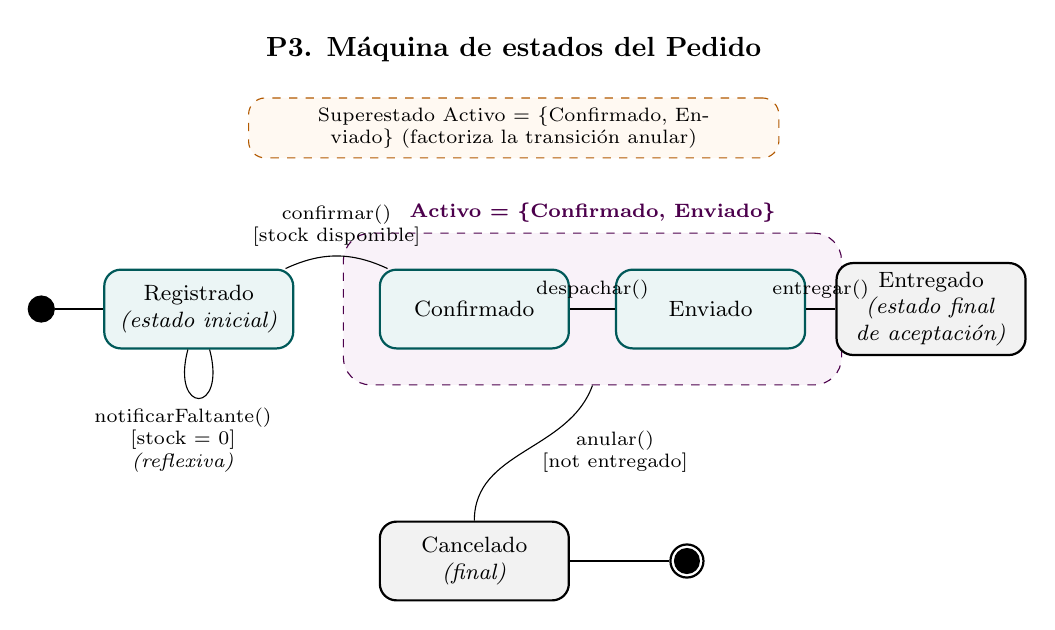
\begin{tikzpicture}[
    state/.style={rectangle, rounded corners=6pt, draw=teal!70!black, thick,
        fill=teal!8, minimum width=2.4cm, minimum height=1cm, align=center, font=\footnotesize},
    finalstate/.style={rectangle, rounded corners=6pt, draw=black, thick,
        fill=gray!10, minimum width=2.4cm, minimum height=1cm, align=center, font=\footnotesize},
    initial/.style={circle, draw=black, fill=black, minimum size=0.3cm},
    finaldot/.style={circle, draw=black, thick, fill=white, minimum size=0.42cm},
    finaldotinner/.style={circle, fill=black, minimum size=0.18cm},
    every edge/.style={draw, -{Stealth[length=2.5mm]}, thick},
    lbl/.style={font=\scriptsize, align=center}
]

% --- Título ---
\node[font=\bfseries] at (6,7.3) {P3. Máquina de estados del Pedido};

% --- Estados principales ---
\node[initial] (ini) at (0,4) {};
\node[state] (registrado) at (2,4) {Registrado\\\textit{(estado inicial)}};
\node[state] (confirmado) at (5.5,4) {Confirmado};
\node[state] (enviado) at (8.5,4) {Enviado};
\node[finalstate] (entregado) at (11.3,4) {Entregado\\\textit{(estado final}\\\textit{de aceptación)}};

\node[finalstate] (cancelado) at (5.5,0.8) {Cancelado\\\textit{(final)}};
\node[finaldot] (finC) at (8.2,0.8) {};
\node[finaldotinner] at (finC) {};

% --- Superestado Activo ---
\begin{scope}[on background layer]
\node[draw=violet!60!black, dashed, rounded corners=10pt, fill=violet!5,
    fit=(confirmado)(enviado), inner sep=0.45cm, label={[font=\scriptsize\bfseries, violet!60!black]above:Activo = \{Confirmado, Enviado\}}] (activo) {};
\end{scope}

\node[draw=orange!70!black, dashed, rounded corners=6pt, fill=orange!5,
    text width=6.5cm, align=center, font=\scriptsize] at (6,6.3)
    {Superestado Activo = \{Confirmado, Enviado\} (factoriza la transición anular)};

% --- Transiciones ---
\draw (ini) -- (registrado);

\draw (registrado) to[bend left=25] node[lbl, above] {confirmar()\\{[stock disponible]}} (confirmado);

\draw (registrado) to[loop below, looseness=8] node[lbl, below, xshift=-0.2cm]
    {notificarFaltante()\\{[stock = 0]}\\\textit{(reflexiva)}} (registrado);


\draw (confirmado) -- node[lbl, above] {despachar()} (enviado);
\draw (enviado) -- node[lbl, above] {entregar()} (entregado);

% --- Transición factorizada anular() desde el superestado Activo ---
\draw (activo.south) to[out=250,in=90] node[lbl, right, xshift=0.1cm]
    {anular()\\{[not entregado]}} (cancelado.north);

\draw (cancelado) -- (finC);

\end{tikzpicture}
\end{document}

% ============================================================

\documentclass[tikz,border=10pt]{standalone}
\usepackage{tikz}
\usetikzlibrary{shapes.geometric, positioning, arrows.meta, fit, backgrounds}

\begin{document}
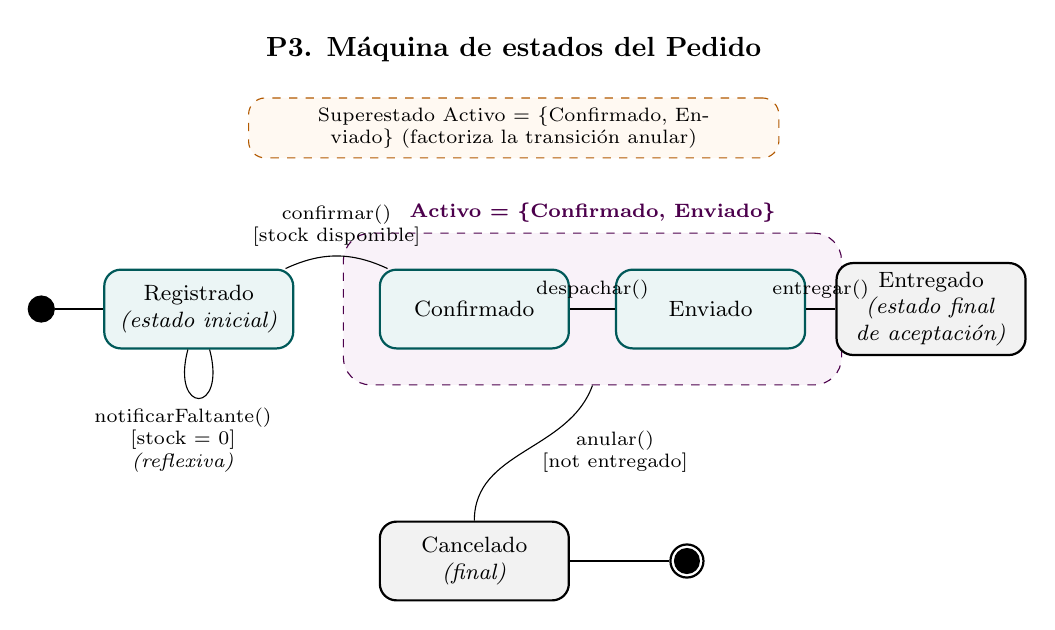
\begin{tikzpicture}[
    state/.style={rectangle, rounded corners=6pt, draw=teal!70!black, thick,
        fill=teal!8, minimum width=2.4cm, minimum height=1cm, align=center, font=\footnotesize},
    finalstate/.style={rectangle, rounded corners=6pt, draw=black, thick,
        fill=gray!10, minimum width=2.4cm, minimum height=1cm, align=center, font=\footnotesize},
    initial/.style={circle, draw=black, fill=black, minimum size=0.3cm},
    finaldot/.style={circle, draw=black, thick, fill=white, minimum size=0.42cm},
    finaldotinner/.style={circle, fill=black, minimum size=0.18cm},
    every edge/.style={draw, -{Stealth[length=2.5mm]}, thick},
    lbl/.style={font=\scriptsize, align=center}
]

% --- Título ---
\node[font=\bfseries] at (6,7.3) {P3. Máquina de estados del Pedido};

% --- Estados principales ---
\node[initial] (ini) at (0,4) {};
\node[state] (registrado) at (2,4) {Registrado\\\textit{(estado inicial)}};
\node[state] (confirmado) at (5.5,4) {Confirmado};
\node[state] (enviado) at (8.5,4) {Enviado};
\node[finalstate] (entregado) at (11.3,4) {Entregado\\\textit{(estado final}\\\textit{de aceptación)}};

\node[finalstate] (cancelado) at (5.5,0.8) {Cancelado\\\textit{(final)}};
\node[finaldot] (finC) at (8.2,0.8) {};
\node[finaldotinner] at (finC) {};

% --- Superestado Activo ---
\begin{scope}[on background layer]
\node[draw=violet!60!black, dashed, rounded corners=10pt, fill=violet!5,
    fit=(confirmado)(enviado), inner sep=0.45cm, label={[font=\scriptsize\bfseries, violet!60!black]above:Activo = \{Confirmado, Enviado\}}] (activo) {};
\end{scope}

\node[draw=orange!70!black, dashed, rounded corners=6pt, fill=orange!5,
    text width=6.5cm, align=center, font=\scriptsize] at (6,6.3)
    {Superestado Activo = \{Confirmado, Enviado\} (factoriza la transición anular)};

% --- Transiciones ---
\draw (ini) -- (registrado);

\draw (registrado) to[bend left=25] node[lbl, above] {confirmar()\\{[stock disponible]}} (confirmado);

\draw (registrado) to[loop below, looseness=8] node[lbl, below, xshift=-0.2cm]
    {notificarFaltante()\\{[stock = 0]}\\\textit{(reflexiva)}} (registrado);


\draw (confirmado) -- node[lbl, above] {despachar()} (enviado);
\draw (enviado) -- node[lbl, above] {entregar()} (entregado);

% --- Transición factorizada anular() desde el superestado Activo ---
\draw (activo.south) to[out=250,in=90] node[lbl, right, xshift=0.1cm]
    {anular()\\{[not entregado]}} (cancelado.north);

\draw (cancelado) -- (finC);

\end{tikzpicture}
\end{document}
}
    \caption{Máquina de estados -- Pedido}
    \label{fig:state}
\end{figure}

\newpage

% =========================================================
% P4
% =========================================================
\section{Consistencia entre las tres perspectivas}

\subsection*{Tabla de verificación cruzada}
\begin{center}
\begin{tabular}{lll}
\toprule
\textbf{Evento (P3)} & \textbf{Función/acción (P2)} & \textbf{Entidad/atributo (P1)} \\
\midrule
confirmar & Confirmar pedido & Pedido.estado \\
despachar & Despachar pedido & Pedido.estado \\
entregar  & Entregar pedido  & Pedido.estado \\
anular    & Anular pedido    & Pedido.estado \\
\bottomrule
\end{tabular}
\end{center}

\subsection*{Inconsistencia detectada}
El evento ``notificar faltante'' (P2) no tiene transición correspondiente en P3, ya que el
pedido permanece en estado Registrado.

\subsection*{Corrección}
Se documenta como nota en la máquina de estados que dicho camino no produce cambio de estado
(auto-transición interna en Registrado).

\newpage

% =========================================================
% P5
% =========================================================
\section{Especificación de requisitos con esquema de atributos}

\subsection*{Requisitos funcionales}
\begin{itemize}
    \item \textbf{RF-01}: El sistema debe permitir registrar un pedido con sus líneas y calcular el total automáticamente.
    \item \textbf{RF-02}: El sistema debe verificar el stock del producto antes de confirmar el pedido.
\end{itemize}

\subsection*{Requisitos no funcionales}
\begin{itemize}
    \item \textbf{RNF-01} (Eficiencia de desempeño, ISO/IEC 25010): el sistema debe registrar un pedido en menos de 3 segundos bajo carga normal.
    \item \textbf{RNF-02} (Seguridad, ISO/IEC 25010): los datos personales del cliente deben cifrarse en reposo y en tránsito.
\end{itemize}

\subsection*{Esquema de atributos}
\begin{center}
\begin{tabular}{lllllll}
\toprule
\textbf{ID} & \textbf{Prioridad} & \textbf{Estado} & \textbf{Fuente} & \textbf{Estabilidad} & \textbf{Versión} & \textbf{Verificación} \\
\midrule
RF-01  & Alta  & Propuesto & Caso de negocio & Alta  & 1.0 & Prueba \\
RF-02  & Alta  & Propuesto & Caso de negocio & Alta  & 1.0 & Prueba \\
RNF-01 & Media & Propuesto & Caso de negocio & Media & 1.0 & Prueba de carga \\
RNF-02 & Media & Propuesto & Caso de negocio & Media & 1.0 & Inspección/prueba \\
\bottomrule
\end{tabular}
\end{center}

\newpage

% =========================================================
% P6
% =========================================================
\section{Priorización MoSCoW}

\begin{itemize}
    \item \textbf{RF-01 -- Must have}: es el núcleo funcional del sistema.
    \item \textbf{RF-02 -- Must have}: garantiza integridad de datos e inventario.
    \item \textbf{RNF-01 -- Should have}: mejora la experiencia, pero no bloquea la operación básica.
    \item \textbf{RNF-02 -- Could have}: deseable desde el inicio, puede incorporarse en una iteración posterior.
\end{itemize}

\newpage

% =========================================================
% P7
% =========================================================
\section{Validación por inspección (checklist ISO/IEC/IEEE 29148)}

\subsection*{Propiedades evaluadas}
No ambiguo, completo, singular, verificable, factible.

\subsection*{Defecto detectado (sin corregir)}
RNF-02 no especifica algoritmo ni umbral medible $\rightarrow$ incumple ``verificable''.

\subsection*{Retrabajo (segundo paso)}
``Los datos personales deben cifrarse con AES-256 en reposo y TLS 1.3 en tránsito.''

\newpage

% =========================================================
% P8
% =========================================================
\section{Pruebas de aceptación trazadas}

\begin{center}
\begin{tabular}{p{1.3cm}p{1.8cm}p{3.2cm}p{4.2cm}p{1.5cm}}
\toprule
\textbf{ID} & \textbf{Tipo} & \textbf{Entradas} & \textbf{Criterio de éxito} & \textbf{Traza a} \\
\midrule
PA-01 & Funcional     & Pedido con 2 líneas válidas         & Total calculado correctamente             & RF-01 \\
PA-02 & Funcional     & Producto sin stock                  & Sistema notifica faltante, no confirma    & RF-02 \\
PA-03 & No funcional  & 100 pedidos simultáneos             & Cada registro $<$ 3 s                     & RNF-01 \\
PA-04 & No funcional  & Intento de acceso directo a BD      & Datos ilegibles sin clave                 & RNF-02 \\
\bottomrule
\end{tabular}
\end{center}

\newpage

% =========================================================
% P9
% =========================================================
\section{Matriz de trazabilidad}

\begin{center}
\begin{tabular}{p{1.5cm}p{2.5cm}p{5cm}p{1.7cm}}
\toprule
\textbf{Requisito} & \textbf{Fuente (traza atrás)} & \textbf{Modelo asociado} & \textbf{Prueba (traza adelante)} \\
\midrule
RF-01  & Caso de negocio & P1: Pedido/LíneaPedido; P2: flujo completo   & PA-01 \\
RF-02  & Caso de negocio & P1: Producto.stock; P2: decisión stock       & PA-02 \\
RNF-01 & Caso de negocio & P2: flujo ``Registrar pedido''               & PA-03 \\
RNF-02 & Caso de negocio & P1: Cliente (datos personales)               & PA-04 \\
\bottomrule
\end{tabular}
\end{center}

\subsection*{Dependencia horizontal}
RF-02 depende de RF-01 (no puede verificarse stock sin un pedido creado).

\subsection*{Requisitos huérfanos}
Ninguno; los cuatro requisitos cuentan con modelo y prueba asociados.

\newpage

% =========================================================
% P10
% =========================================================
\section{Gestión del cambio y línea base}

\subsection*{Solicitud de cambio}
``Agregar notificación por correo al cliente al confirmar el pedido''.

\subsection*{Análisis de impacto (según matriz P9)}
Afecta a RF-01, al diagrama de clases (nuevo método en Pedido) y a la prueba PA-01.

\subsection*{Decisión del CCB}
Aprobada, prioridad Should have.

\subsection*{Nueva versión}
RF-01 pasa de v1.0 a v1.1.

\subsection*{Línea base declarada (Baseline 1.0)}
Se congela la configuración coherente: ERS v1.0, modelos de clases/actividades/estados v1.0,
matriz de trazabilidad v1.0 y pruebas de aceptación v1.0.

\newpage

% =========================================================
% ANEXO -- EVIDENCIA DE EVALUACIÓN EN EL SGA
% =========================================================
\section*{Anexo -- Evidencia de la evaluación en el SGA}
\addcontentsline{toc}{section}{Anexo -- Evidencia de la evaluación en el SGA}

\begin{figure}[h!]
    \centering
    \includegraphics[width=\linewidth]{img1.jpg}
    \caption{Resumen del cuestionario -- Evaluación Sumativa Unidad IV}
\end{figure}

\begin{figure}[h!]
    \centering
    \includegraphics[width=\linewidth]{img2.jpg}
    \caption{Revisión de intento -- Ingeniería de Requerimientos}
\end{figure}

\end{document}
